\documentclass[12pt]{article}

% Layout.
\usepackage[top=1in, bottom=0.75in, left=1in, right=1in, headheight=1in, headsep=6pt]{geometry}

% Fonts.
\usepackage{mathptmx}
\usepackage[scaled=0.86]{helvet}
\renewcommand{\emph}[1]{\textsf{\textbf{#1}}}

% TiKZ.
\usepackage{tikz, pgfplots}
\usetikzlibrary{calc}

% Misc packages.
\usepackage{amsmath,amssymb,latexsym}
\usepackage{graphicx}
\usepackage{array}
\usepackage{xcolor}
\usepackage{multicol}
\usepackage{fancyhdr}
\pagestyle{fancy}


% Misc.
\renewcommand{\d}{\displaystyle}
\newcommand{\ds}{\displaystyle}
\def\bc{\begin{center}}
\def\ec{\end{center}}
\def\be{\begin{enumerate}}
\def\ee{\end{enumerate}}

\newcommand{\ans}[1][1in]{\rule{#1}{.5pt}}


\lhead{Math F113X: Quiz 6}

\begin{document}

\vspace{1cm}

\noindent \textbf{Name:} \hrulefill \quad  score:\ans[1cm] \ / 10 \\


There are 10 points possible on this quiz. No aids (book, notes, etc.)
are permitted. You may use a non-programmable calculator.  {\bf Show
all work and supporting calculations for full credit. Explain how you
get your answers.}

\be
\item Consider the following graph.

  \begin{center}
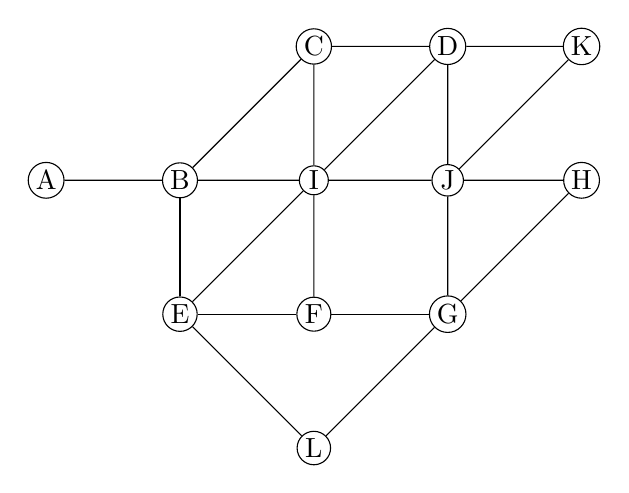
\begin{tikzpicture}[
    baseline=(current bounding box.center),
    lbl/.style={inner sep=2pt, fill=white},
    scale=1.7
]
\tikzstyle{vertex}=[circle, draw, inner sep=1pt]
\tikzstyle{every node}=[vertex]

\node (a) at (-1,1) {A};
\node (b) at (0,1) {B};
\node (c) at (1,2) {C};
\node (d) at (2,2) {D};
\node (e) at (0,0) {E};
\node (f) at (1,0) {F};
\node (g) at (2,0) {G};
\node (h) at (3,1) {H};
\node (i) at (1,1) {I};
\node (j) at (2,1) {J};
\node (k) at (3,2) {K};
\node (l) at (1,-1) {L};

\foreach \u/\v in {a/b,b/c,b/e,b/i,c/d,c/i,d/i,d/k,d/j,e/f,e/i,e/l,f/g,f/i,g/h,g/j,g/l,h/j,i/j,j/k}{\draw (\u) -- (\v);}
\end{tikzpicture}
\end{center}

\be
\item (2 point) This graph does \emph{not} contain an Euler circuit. How can you tell?
  \vfill

\item (3 points) \emph{Eulerize} the graph \emph{using as few edge duplications as possible}. You may do so on the graph provided above, but you must also list your duplicated edges below. 

Another copy of the graph is provided below in case you need to make corrections. If you do work on both graphs, please \textit{clearly indicate which one contains your final answer}.

\bigskip

\emph{Write your duplicated edges here:} \hrulefill
  
  \begin{center}
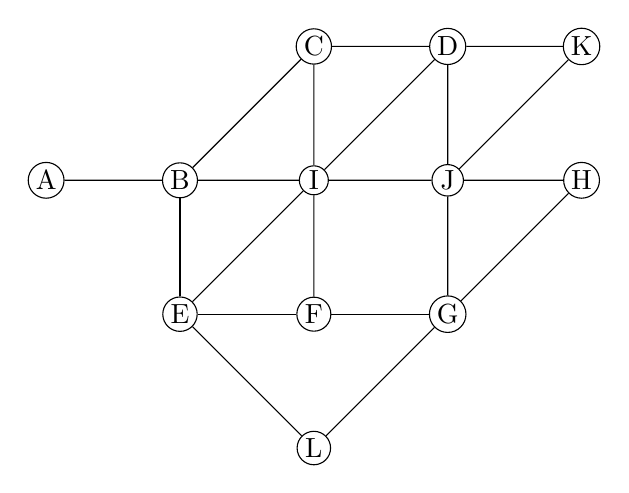
\begin{tikzpicture}[
    baseline=(current bounding box.center),
    lbl/.style={inner sep=2pt, fill=white},
    scale=1.7
]
\tikzstyle{vertex}=[circle, draw, inner sep=1pt]
\tikzstyle{every node}=[vertex]

\node (a) at (-1,1) {A};
\node (b) at (0,1) {B};
\node (c) at (1,2) {C};
\node (d) at (2,2) {D};
\node (e) at (0,0) {E};
\node (f) at (1,0) {F};
\node (g) at (2,0) {G};
\node (h) at (3,1) {H};
\node (i) at (1,1) {I};
\node (j) at (2,1) {J};
\node (k) at (3,2) {K};
\node (l) at (1,-1) {L};

\foreach \u/\v in {a/b,b/c,b/e,b/i,c/d,c/i,d/i,d/k,d/j,e/f,e/i,e/l,f/g,f/i,g/h,g/j,g/l,h/j,i/j,j/k}{\draw (\u) -- (\v);}
\end{tikzpicture}
\end{center}
  \ee
  
\newpage

\item Consider the following graph.

\begin{center}
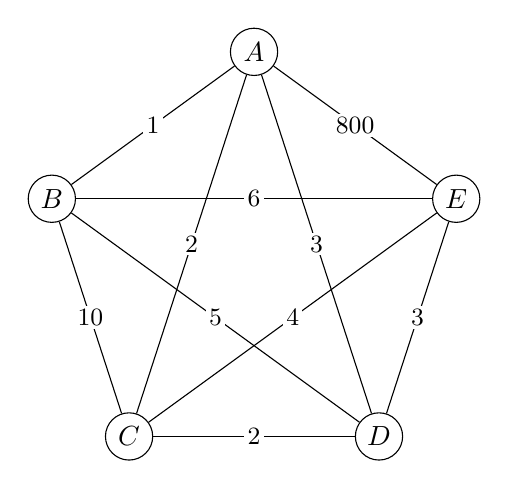
\begin{tikzpicture}[scale = 0.9,
    vertex/.style={circle, draw=black, minimum size=6mm, inner sep=0pt},
    weight/.style={font=\small, fill=white, inner sep=1.2pt}
]
    \def\n{5}
    \def\radius{3cm}
    \foreach \i/\l in {1/A, 2/B, 3/C, 4/D, 5/E} {
        \node[vertex] (v\i) at ({360/\n * (\i - 1) + 90}:\radius) {$\l$};
    }
    % Edges from A
    \draw (v1) -- node[weight] {1} (v2);
    \draw (v1) -- node[weight] {2} (v3);
    \draw (v1) -- node[weight] {3} (v4);
    \draw (v1) -- node[weight] {800} (v5);
    % Edges from B
    \draw (v2) -- node[weight] {10} (v3);
    \draw (v2) -- node[weight] {5} (v4);
    \draw (v2) -- node[weight] {6} (v5);
    % Edges from C
    \draw (v3) -- node[weight] {2} (v4);
    \draw (v3) -- node[weight] {4} (v5);
    % Edges from D
    \draw (v4) -- node[weight] {3} (v5);
\end{tikzpicture}
\end{center}

  \be

\item (3 points) Use the \emph{Nearest Neighbor} (NN) algorithm starting at vertex
  A to find a  Hamiltonian circuit. You should draw your circuit below, and also give your answer as a list of vertices, along with the total weight.

  \begin{center}
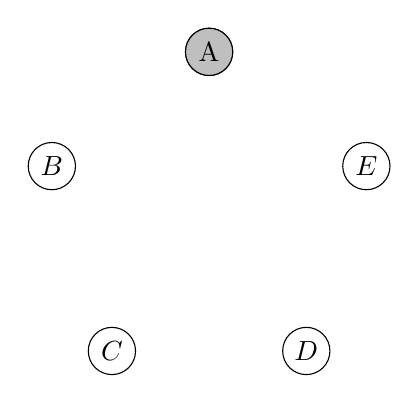
\begin{tikzpicture}[scale = 0.7,
    vertex/.style={circle, draw=black, minimum size=6mm, inner sep=0pt},
    weight/.style={font=\small, fill=white, inner sep=1.2pt}
]
    \def\n{5}
    \def\radius{3cm}
    \foreach \i/\l in {1/A, 2/B, 3/C, 4/D, 5/E} {
        \node[vertex] (v\i) at ({360/\n * (\i - 1) + 90}:\radius) {$\l$};
    }
    \path (v1) node[vertex, fill = gray!50] {A};
\end{tikzpicture}
\end{center}
  

\noindent
Circuit (List vertices):\underline{\hskip 3.in}

\ 

\noindent
Total weight of circuit:\underline{\hskip 3.in}

\bigskip

\item (2 points) Can you find a lower weight Hamiltonian circuit than the one you
found in part (a)? If so, draw the circuit below, list the vertices in order, and
state the total weight. If not, explain why it is not possible.

\begin{tikzpicture}[scale = 0.7,
    vertex/.style={circle, draw=black, minimum size=6mm, inner sep=0pt},
    weight/.style={font=\small, fill=white, inner sep=1.2pt}
]
    \def\n{5}
    \def\radius{3cm}
    \foreach \i/\l in {1/A, 2/B, 3/C, 4/D, 5/E} {
        \node[vertex] (v\i) at ({360/\n * (\i - 1) + 90}:\radius) {$\l$};
    }
\end{tikzpicture}
  \ee
  
  Cheaper circuit, if possible (list vertices): \hrulefill Total Weight \ans[1cm]
  
\ee
\end{document}
%%% Local Variables:
%%% mode: LaTeX
%%% TeX-master: t
%%% End:
